\chapter{Research Framework\label{cha:method}}
%823words
The main purpose of this chapter is to describe a research approach used in this
study. The first section of the chapter identifies the objectives that need to
be addressed in order to achieve the goal of this study, followed by the research
questions in Section \ref{sec:questions} raised from these objectives.

Design Science Research (DSR) methodology was adopted as the main research
methodology of this study to address the research questions. This methodology
emphasizes the problem-solving and performance-improving paradigms and is
oriented towards creating and evaluating IT artifacts \citep{Hevner2004}. A
six-stage research project framework is outlined in Section \ref{sec:method}
which explains each stage of the project and the methods applied. Methodological
limitations are brought to considerations in Section \ref{sec:limits}. This
chapter concludes with the discussion of related work and projects carried out
in the area of \LLLsn.

\section{Research Objectives}

Understanding what kind of technical solution is required to effectively support
\LLLs in universities is an overarching goal of this research. This goal brings
up a number of objectives that need to be addressed:
\begin{description}
  \item[Objective 1.] To determine student and institutional requirements for a
  \LLLs environment within the university context;
  \item[Objective 2.] To map these requirements against the systems already used
  in universities to support \LLLsn;
  \item[Objective 3.] To design and implement the features required in an
  environment that supports \LLLs to satisfy the defined requirements;
  \item[Objective 4.] To evaluate how this environment meets the needs of all
  stakeholders in supporting \LLLsn.
\end{description}

\section{Research Questions}
\label{sec:questions}
Based on the context of the research objectives, this study addressed the
following research questions supported by sub-questions:

\begin{description}
  \item[RQ1:] \textit{What is the concept of \LLLs and its connection to the
  universities?}
	\begin{itemize}
	  \item What is the role of \LLLs in the university context?
	  \item What is the motivation of universities in supporting \LLLsn?
  	  \item What are the existing university policies for supporting \LLLsn?
      \item What are the components of \LLLs environments in universities?
      \item What are the requirements for successful \LLLs support in
   universities?
	\end{itemize} 
	
   \item[RQ2:] \textit{What e-tools are available to support \LLLs within the
   university context?}
	\begin{itemize}
		\item What e-tools are available to support \LLLsn:
			\begin{itemize}
				\item in general?
				\item in universities?
			\end{itemize}
		\item What are the conceptual strengths and weaknesses of these e-tools in
university context?
		\item What is the relationship between LMS and e-tools support for \LLLs in
university context?
	\end{itemize}

	\item[RQ3:] \textit{How can LMS and/or ePortfolio systems be extended to
	support students in a university context in \LLLsn?}
	\begin{itemize}
		\item What features are available now in these systems?
		\item What are the students and institutional requirements for LMS and
		ePortfolio to support \LLLsn?
		\item How can these requirements be translated and implemented into new or
		improved features?
	\end{itemize}

	\item[RQ4:] \textit{Do this extended environment meet the needs of the
	stakeholders in university teaching and learning contexts?}
	\begin{itemize}
		\item How can lecturers use new features to provide students with their
guidance and help them to understand \LLLs skills?
		\item How can students address institutional graduate attributes and other
		skills using new features?
		\item How can new features help students track their learning progress, manage
ePortfolio knowledge and content, demonstrate and share their achievements
with others?
	\end{itemize}
\end{description}

\section{Research Approach}
\label{sec:method}

Finding the most efficient research approach is an important part of any
research study. A properly selected approach helps to obtain answers to the
research questions while working within the framework that uses methods that
have been verified and tested for validity \citep{Kumar2005}. Multi-paradigmatic
field of ICT offers a number of methodologies drawn from the variety of research
philisophies \citep{Vaishnavi2007}. This study follows design science research
methodology that has become popular over the last five decades as fundamentally
a problem-solving appoach \citep{Cross1993}.

\subsection{Design Science Research Methodology}

According to \citet{Peffers2008}, design science research (DSR) originates from
engineering and computer science where design is a component of the research
process. \citet{Iivari2009} define DSR as \inlinequote{a research activity that
invents or builds new, innovative artifacts for solving problems or achieving
improvements}. This approach is used in ICT where there is a need to extend the
existing boundaries of current systems or address the important problems by
creating new and innovative solutions and artifacts \citep{Hevner2004}. The
artifacts can be described as constructs (vocabulary of a domain), methods
(algorithms), models (abstractions), instantiations (prototype systems), and
better theories \citep{Hevner2010}.

Requirements for DSR contribution, defined by \citet{March2008}, include (1)
identification of a problem, (2) demonstration that there are no existing
adequate solutions in the area, (3) development of an innovative artifact that
addresses the problem, (4) evaluation of the artifact, (5) communication of the
knowledge added to the area, and (6) understanding of the implications for
theory and practice.

This set of requirements closely resembles the DRS methodology process described
by \citet{Peffers2008} (see Figure \ref{fig:peffers}) and research model phases
found in \citet{Vaishnavi2007} (see Figure \ref{fig:vaishnavi}).

\begin{figure}[h!]
\centering
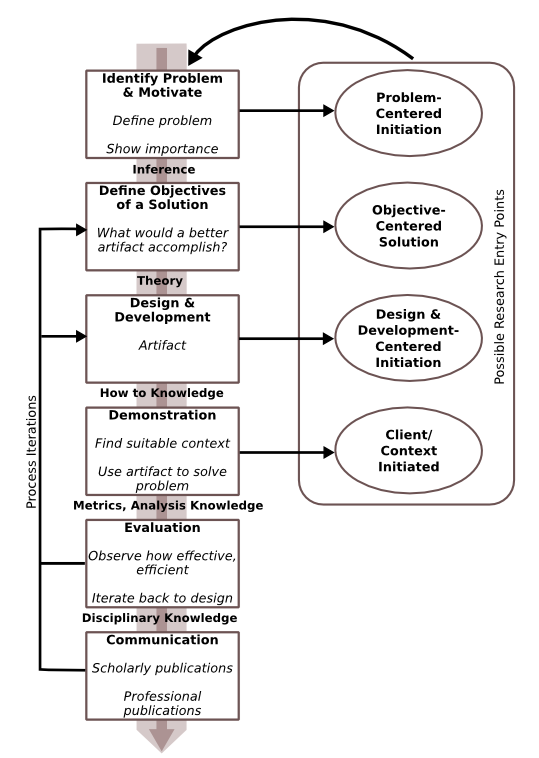
\includegraphics[height=0.75\textheight]{CH2-F1-Peffers}
\caption[Design Science Research Methodology Process Model]{Design Science
Research Methodology Process Model \citep{Peffers2008}}
\label{fig:peffers}
\end{figure}

\FloatBarrier

\begin{figure}[htp]
\centering
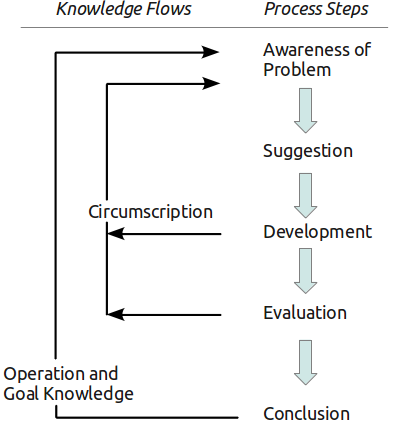
\includegraphics[width=0.5\textwidth]{CH2-F2-Vaishnavi}
\caption[Design Science Reseach Cycle]{Design Science Reseach Cycle
\citep{Vaishnavi2007}}
\label{fig:vaishnavi}
\end{figure}

All authors essentially agree on common elements. The initial stage of research
is \textit{problem identification} or awareness where a specific research
problem should be stated and the importance of its solution should be justified.
After the problem is identified, next step is to \textit{suggest a solution} and
define its objectives. This includes understanding the state of the problem and
current available solutions, if any, and explaining how new solution is going to
address the problem in a better way. 

\FloatBarrier

The core phase of research is \textit{design and development}. Conceptually,
this phase consists of deciding the artifact's functional requirements or its
architecture and afterwards creating artifact itself. \citet{Peffers2008} note
that in some cases an artifact is not necessarily a new development. It might
have been already used in another research domain to solve a different problem.

Unlike Vaishnavi's research cycle where evaluation is one step of research
process, Peffer's model distinguishes between \textit{demonstration} and
\textit{evaluation} of the artifact. Demonstration is used to show that the
implemented idea works, while evaluation is more formal form of measuring how
well the artifact supports a solution to the problem \citep{Peffers2008}.
Artifact can be evaluated from various perspectives such as performance,
usability, reliability, accuracy, quality, functionality, etc.

The last stage of research is \textit{conclusion} or \textit{communication}. It
might involve but is not limited to: discussing the problem, its importance, the
novel artifact, and its effectiveness with relevant research audiences; creating
scholarly publications; presenting research findings at the conferences; and
writing a project report \citep{Archer1984}. However, if no satisfying results
have been reached at this stage of the research cycle, it might as well serve as
a subject for further reseach.

To assist beginning researches, Hevner \citeyearpar{Hevner2004} identifies seven
guidelines to follow for effective DSR:

\begin{table}[htb]
  \begin{center}
    \begin{tabular}{| l | p{6.5cm} |}
    \hline
     \multicolumn{1}{|c|}{\textbf{Guidelines}} &
     \multicolumn{1}{c|}{\textbf{Description}} \\
     \hline
     Guideline 1: Design as an Artifact & Research must produce a viable
    artifact such as a construct, a model, a method or an instantiation \\ \hline
     Guideline 2: Problem Relevance & Research must develop technology-based
     solutions to important and relevant problems \\ \hline 
     Guideline 3: Design Evaluation & Proper valuation mthods must be used to
     demonstrate artifact's quality and efficacy \\ \hline 
     Guideline 4: Research Contributions & Research must provide clear
     contributions to the research areas \\ \hline 
     Guideline 5: Research Rigor & Rigorous methods must be applied to
     construction and evaluation of the artifacts \\ \hline 
     Guideline 6: Design as a Search Process & Research must incorporate a
     search process to find and effective solution to the problem \\ \hline
     Guideline 7: Communication of Research & Research must be effectivey
     communicated to relevant audiences \\ \hline
    \end{tabular}
  \end{center}
  \caption{Design Science Research Guidelines \citep{Hevner2004}}
\end{table}

In contrast to Hevner, \citet{Venable2010} argues that there is no common
understanding of what kind of guidelines and standards should be used for
effective DSR. However, based on analysis in the same work, the majority of
researchers and DSR practitioners agree on a few points: DSR should address
important problems, have an artifact that would help to solve the problem, and
have some kind of evaluation of this artifact.

\subsection{Design Science Research Applied to This Project}

The research framework in the current research is adapted from a DSR cycle
established by \citet{Vaishnavi2007}. They identify five phases in the research
model: (a) awareness of a problem, (b) suggestions of solution, (c) development,
(d) demonstration and evaluation, and (e) conclusion and communication.

\subsubsection{Stage 1. Problem identification and motivation}

The problem identified in the current research is not efficient technical
support for \LLLs in universities.

\subsubsection{Stage 2. Objectives for a Solution}

To answer the reseach question on the concept of \LLLs and what tools can be
used to support it, it is important to develop understanding of current
situation and practices of \LLLs support. A comprehensive literature review
and a review of the learning spaces was undertaken to address these questions.
However, this research did not rely on a literature review alone. A set of
interviews with the stakeholders were organized to support literature finidings
and identify the gaps that exsist in current \ep~systems.

\subsubsection{Stage 3. Design and Development}

In the development phase, the results of the literature review, interviews and
requirements analysis were used to create a conceptual model of an \ep-supported
environment which can facilitate students in \LLLs and be compatible with
university needs.

A functionality, based on this model, was implemented in a prototype \ep~system.
As requirements specifications was too large for the project of such size and
relatively short timeline, only priority requirements were implemented. The
requirements were prioritized according to the feedback given by the interviews
participants at the initial stages of the project. Due to this, a set of
requirements for a better integration of the \ep~systems with LMS was left
behind. Although, these requirements were not implemented they were still
included into the conceptual model.

Prototyping followed established software engineering practices that interleaved
coding and revision, forming iterative development cycles, as it shown at
\ref{fig:prototype}.

\begin{figure}[htb]
\centering
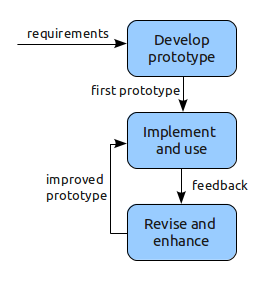
\includegraphics[height=0.3\textheight]{CH2-F3-Prototype}
\caption[Ptototyping]{Prototyping based on \citet*[p.~411]{Sommerville2007}}
\label{fig:prototype}
\end{figure}

Mahara \ep~system was used as an initial base system for a prototype. There
are a number of reasons why this system was selected. Mahara is trusted,
widely-used in universities (and at Massey University in particular) solution
with a large community support. This system is open source which makes it easy
to access and allows modifications like adding new features and changing the
existing ones. Mahara is a \textit{typical} representative of its category and
provides all commonly available features. At the same time it is a leading edge
system developed by using latest web technologies and programming practice.

After each iteration was completed, the stakeholders were consulted for feedback
and design of further improvements. 



\subsubsection{Stage 4. Demonstration and Evaluation}

It is important for evaluation to be treated not as an isolated process, but as
a part of design process \citep{Cleven2009}.

Due to the context of this research -- \LLLsn, -- it had a complex evaluation
design. 

Case studies were used to evaluate prototype from the mature students
perspective. This approach was favoured over others due to its internal and
external validity, control and in-depth examination of each case
\citep{Yin2009}.

\subsubsection{Stage 5. Conclusion and Communication}

Where possible the results of the various stages of this research project were
documented and submitted for publications and conference presentations. Full
list of publications can be found in \hyperref[sec:pub]{Publications and
Presentations} section of this thesis.

\section{Methodological Limitations}
\label{sec:limits}

Any study and its findings should be weighed against methodological limitations.
Acknowledging limitations is important for scientific progress as they might help
to understand how research can be improved in the future \citep{Ioannidis2007}.
Although, literature does not provide the explicit list of limitations of DSR
methodology, they can still be derived from the limitations of methods used at
each stage of the study. Therefore, the limitations considered in this research
included:

\begin{description}
\item[Literature:] No explicit requirements for \LLLs support on a system level;
\item[Sample size:] Sample size was relatively small due to the participants
profile requirements;
\item[Prototyping:] Evaluated system was a prototype based on open source
\ep~system Mahara which might have led to biased feedback as some participant
were familiar with the system and already had their opinion about it;
\item[Evaluation design:] Developing evaluation design was restricted by the
scale of this research project, its time and resources constraints; 
\item[Something else:]
\end{description}

More detailed analysis of limitations is discussed further in the relevant
chapters.

\section{Related Work}
\label{sec:related}
As the field of \LLLs became popular, there were a number of studies aimed to
explore \LLLs support in various contexts. To date, research similar to this
project has not been identified, although projects found were a valuable source
of information and examples of previous research experience.

\begin{itemize}

  \item Lifelong Learning in London for
  All\footnote{\url{http://www.lkl.ac.uk/research/l4all.html}} (L4All): This
  project is focused on developing of \LLLs system to support independent
  learners (particularly those 16+ learners who traditionally have not
  participated in higher education) by recording their learning pathways. This
  project aimed to provide lifelong learners in the London region with access to
  information and resources that facilitates their progression from secondary
  education to further education or from secondary education directly to higher
  education \citep{Freitas2006};

  \item The Regional Interoperability Project on Progression for Lifelong
Learning\footnote{\url{http://www.jisc.ac.uk/whatwedo/programmes/edistributed/rippll.aspx
}} (RIPPLL): This project was going to establish a model of cross-sector
collaboration in personal development planning technology in the UK. The aim was
to make interoperable all the major existing electronic systems for study-based
progress files in use in further and higher education to provide an easier
transition process from school to further education \citep{Hartnell-Young2006};

  \item ELGG-Moodle: In autumn 2006 Klagenfurt University, Austria was piloting
the project aimed to integrated Moodle LMS and ELGG platform. This integration
was used for professional development for all academic staff. Project outcomes
provided integration between systems such as single login and file transfer
\citep{Attwell2007}.

  \item Accessible \LLLc for Higher
Education\footnote{\url{http://www.eu4all-project.eu}} (EU4ALL): a project
started in 2006 and aimed to develop components and services for universities to
make learning more accessible for both the students with functional diversity
and the elderly. This project looks into provididing a better access to the
electronic content and educational resources in higher education using a
framework or a set of free tools that support mobile learning, audio recording
transcription, DAISY digital books and other adaptations of contents based on
the student's needs and preferences.

\end{itemize}

\section{Summary}

This chapter explained the main research approach emplyed in this study to
address the research questions.

Next chapter will look into the theory of \LLLs and how it is described in the
literature that is used later to develop a basis for the study explorations.
